\section{Report Generation}

\subsection{Generating Reports}

If you should so wish it is possible to generate an XML version of the current state the application is in. This report will show you an overview of all your projects, teams, skills, people, team allocations etc so that you can get a general feel for everything in the current state.

To reduce the size of the generated XML file not all information is explicitly added to all parts of the report. It instead is linked in other parts of the report. This prevents the duplication of data.//
If using this report to import into another application, some preproccessing will need to be done to link data together.

In order to generate this report all you need to do is click on File/Generate Report. This will bring a up Report Generation Dialog which defaults to All. On this setting a complete report will be generated. Clicking generate report will bring up a save dialog asking you where you would like to save the report to. Also the save dialog defaults to XML, but if you want you can save it as a .report file. Once you have selected a location and pressed save then if you go to the location that you saved the report in and open the file you will have an XML representation of the file as shown in the diagram below.

\begin{figure}[H]
\centering
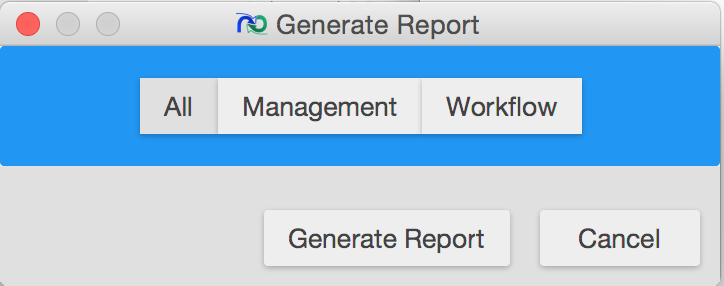
\includegraphics[width=\textwidth]{images/screenshots/report1.PNG}
\caption{Report Generation}
\label{fig:generate_report_all}
\end{figure}

\subsection{Generating Workflow Reports}

A workflow report will only be able to report things that pertain to work flow i.e. Backlogs or Stories. To generate the report, select a type from the report types. And then select one or more items in the list presented. This can be achieved by holding the CTRL key while clicking on the items in the list you want to the report to contain. The Generate Report button works the same as described in the Generating Reports section.

\begin{figure}[H]
\centering
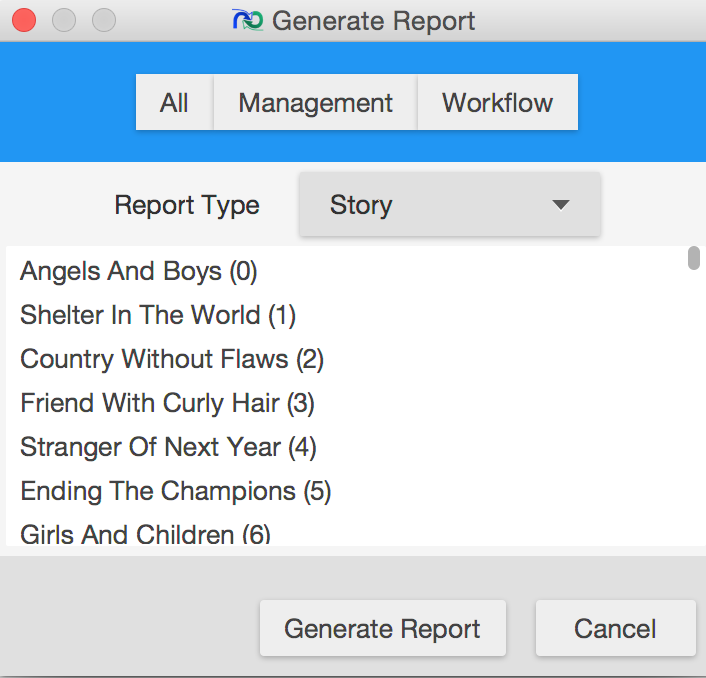
\includegraphics[width=\textwidth]{images/screenshots/report3.PNG}
\caption{Workflow Report Generation}
\label{fig:generate_report_workflow}
\end{figure}

\subsection{Generating Management Reports}

A management report will only be able to report things that pertain to management i.e. Projects, Teams, Persons. To generate the report, select a type from the report types. And then select one or more items in the list presented. This can be achieved by holding the CTRL key while clicking on the items in the list you want to the report to contain. The Generate Report button works the same as described in the Generating Reports section.

\begin{figure}[H]
\centering
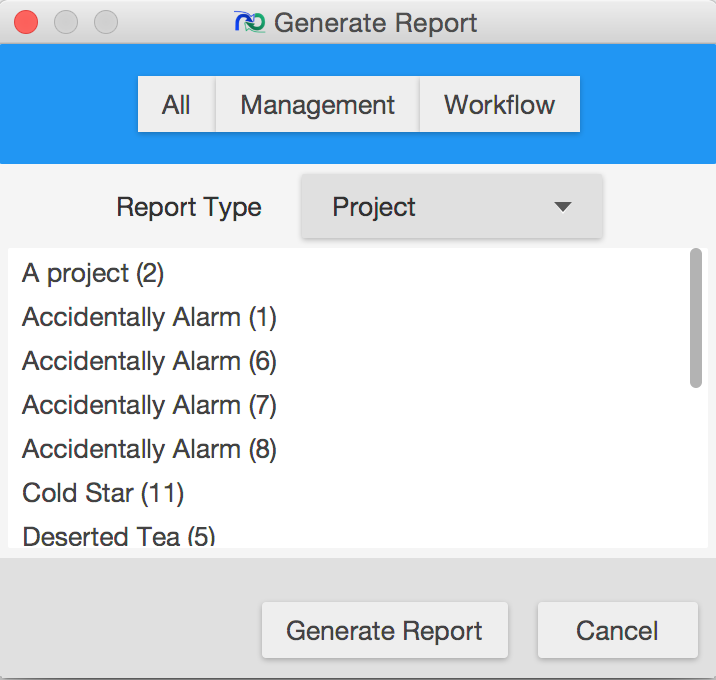
\includegraphics[width=\textwidth]{images/screenshots/report2.PNG}
\caption{Management Report Generation}
\label{fig:generate_report_management}
\end{figure}
